\documentclass[11pt,letterpaper]{article}
\usepackage[utf8]{inputenc}
\usepackage[T1]{fontenc}
\usepackage[spanish,es-nodecimaldot]{babel}
\usepackage{helvet}
\renewcommand{\familydefault}{\sfdefault}
\usepackage[letterpaper,top=2.2cm,bottom=2.2cm,left=2.5cm,right=2.5cm]{geometry}
\usepackage{microtype}
\usepackage{graphicx}
\usepackage{xcolor}
\usepackage{booktabs}
\usepackage{array}
\usepackage{tabularx}
\usepackage{float}
\usepackage{caption}
\usepackage{titlesec}
\usepackage{tikz}
\usepackage{amsmath}
\usepackage{amssymb}
\usepackage{siunitx}
\usepackage{hyperref}
\usepackage{placeins}

% Metadatos editables antes de entregar al cliente.
\newcommand{\ReportID}{EVX-HUEIHUE-2026}
\newcommand{\CageID}{s.d.}
\newcommand{\ReportMonth}{julio/ 2026}

\definecolor{reportblue}{RGB}{36,112,190}
\definecolor{darkblue}{RGB}{31,78,121}
\definecolor{lamporange}{RGB}{237,125,49}
\definecolor{evoluxyellow}{RGB}{253,195,46}
\definecolor{evoluxblack}{RGB}{6,4,0}
\definecolor{evoluxgray}{RGB}{107,107,107}
\hypersetup{colorlinks=true,linkcolor=reportblue,urlcolor=reportblue,citecolor=reportblue}
\captionsetup{font=small,labelfont={color=reportblue},textfont={color=reportblue},justification=centering}
\titleformat{\section}{\bfseries\color{reportblue}\large}{\thesection.}{0.45em}{}
\titleformat{\subsection}{\bfseries\color{reportblue}\normalsize}{\thesubsection}{0.45em}{}
\titlespacing*{\section}{0pt}{1.3em}{0.65em}
\titlespacing*{\subsection}{0pt}{1.0em}{0.5em}
\setlength{\parindent}{1.25cm}
\setlength{\parskip}{0.35em}
\renewcommand{\arraystretch}{1.12}
\pagestyle{empty}
\sisetup{output-decimal-marker={,}}

\begin{document}

\begin{titlepage}
\centering
\makebox[\textwidth][c]{%
\begin{minipage}[c]{0.40\textwidth}
  \centering
\includegraphics[width=\linewidth,height=2.5cm,keepaspectratio]{figures/biomasa-maqsur.jpg}
\end{minipage}
\hspace{0.8cm}
\begin{minipage}[c]{0.40\textwidth}
  \centering
\includegraphics[width=\linewidth,height=2.5cm,keepaspectratio]{figures/evolux-logo.png}
\end{minipage}}

\vspace{4.4cm}
{\LARGE INFORME DE IRRADIANCIA\par}
\vspace{0.8cm}
{\Large Centro de cultivo de Mar ``HUEIHUE''\par}

\vspace{2.3cm}
\begin{minipage}{0.63\textwidth}
\raggedright
{\large Informe: \ReportID\par}
\vspace{0.55cm}
{\large Cliente: MOWI\par}
\end{minipage}

\vfill
{\bfseries \ReportMonth\par}
\end{titlepage}

\section{INTRODUCCIÓN}

La luz, a través de sus ritmos diarios y estacionales, actúa como agente coordinador de procesos biológicos de los salmónidos, regulando eventos fisiológicos como el ciclo reproductivo, el crecimiento, la actividad locomotora y las transiciones de cada etapa vital. En salmón del Atlántico, el fotoperíodo es percibido por fotorreceptores pineales y transducido en señales rítmicas de melatonina, sensibles tanto a la intensidad como al contenido espectral, especialmente en el rango azul-verde (Migaud \emph{et al.}, 2007; Vera \emph{et al.}, 2010).

En ambientes productivos, la aplicación de luz artificial se utiliza para retardar la maduración sexual y potenciar el crecimiento. Leclercq \emph{et al.} (2011) y Oppedal \emph{et al.} (1997) señalan que irradiancias iguales o superiores a \SI{0.012}{\watt\per\square\metre} han sido capaces de evitar la maduración de esta especie. Este valor se utiliza en el presente informe como referencia de irradiancia biológicamente efectiva.

Leclercq \emph{et al.} (2011) sugieren además que el control de la maduración puede lograrse proporcionando un volumen mínimo de irradiancia efectiva equivalente al 12\% del ambiente de cultivo. Ante estos antecedentes, conocer la distribución de la luz al interior de las unidades de cultivo aporta información para definir estrategias productivas consistentes en el tiempo.

\section{OBJETIVOS}

\subsection{Objetivo General}

Determinar la distribución de irradiancia en una jaula de engorda de salmón del Atlántico del centro Hueihue e identificar potenciales niveles de iluminación fuera de los rangos recomendados por la literatura.

\section{Materiales y métodos}

Durante la noche del 9 al 10 de julio de 2026 se realizaron mediciones en un cuadrante de una jaula de cultivo de salmón del Atlántico, cuadrada y de \SI{50}{\metre} por lado. La unidad fue iluminada con ocho lámparas Tempest operadas a \SI{650}{\watt} cada una, con potencia eléctrica total de \SI{5200}{\watt}. Las fuentes se encontraban instaladas a una profundidad nominal de \SI{3}{\metre}.

\subsection{Procedimiento general}

Se aplicó simetría espacial sobre el cuadrante comprendido por $x,y\in\{6,12,18,24\}$ m. Se midieron dos profundidades, $z\in\{8,10\}$ m, totalizando 32 posiciones. Las coordenadas corresponden a distancias desde una esquina de la jaula.

\begin{figure}[H]
\centering
\begin{tikzpicture}[x=0.084cm,y=0.084cm]
  \fill[evoluxyellow!18] (0,0) rectangle (25,25);
  \draw[thick] (0,0) rectangle (50,50);
  \foreach \t in {0,10,20,30,40,50}{
    \draw (\t,0)--(\t,-0.8);
    \node[anchor=north,font=\scriptsize] at (\t,-1.2) {\t};}
  \foreach \t in {10,20,30,40,50}{
    \draw (0,\t)--(-0.8,\t);
    \node[anchor=east,font=\scriptsize] at (-1.2,\t) {\t};}
  \draw[dashed,evoluxgray] (25,0)--(25,25)--(0,25);
  \foreach \x in {6,12,18,24}{\foreach \y in {6,12,18,24}{\fill[evoluxblack] (\x,\y) circle (0.65);}}
  \foreach \x/\y in {12.5/12.5,37.5/12.5,12.5/25,37.5/25,12.5/37.5,37.5/37.5,25/16.5,25/33.5}{
    \fill[evoluxyellow] (\x,\y+1.0)--(\x-1.0,\y-0.9)--(\x+1.0,\y-0.9)--cycle;}
  \node[anchor=west] at (52,34) {\textcolor{evoluxyellow}{$\blacktriangle$} Lámpara};
  \node[anchor=west] at (52,28) {\textcolor{evoluxblack}{$\bullet$} Medición};
  \node[anchor=west] at (52,22) {Cuadrante muestreado};
  \node at (25,-8.0) {$x$ [m]};
  \node[rotate=90] at (-11.0,25) {$y$ [m]};
\end{tikzpicture}
\caption{Esquema de la jaula, cuadrante medido y disposición nominal de las ocho lámparas. Profundidades de medición: 8 y 10 m.}
\end{figure}

Los datos correspondieron a mediciones realizadas con un medidor de irradiancia espectral OHSP-350, capaz de registrar información en el espectro PAR (380--680 nm). Durante la medición, el sensor se orientó mirando hacia arriba. Los valores se expresaron en unidades de irradiancia (W/m$^2$).

\subsection{Identificación general de las unidades de cultivo}

\begin{table}[H]
\centering
\caption{Identificación del ambiente de cultivo e iluminación de la unidad evaluada.}
\begin{tabularx}{0.72\textwidth}{>{\raggedright\arraybackslash}X >{\centering\arraybackslash}p{4.8cm}}
\toprule
Datos & Jaula \\
\midrule
ID. jaula & \CageID \\
Tipo jaula & Cuadrada \\
Lado (m) & 50 \\
Profundidad relinga inferior (m) & s.d. \\
Especie & Salmón Atlántico (\emph{S. salar}) \\
Densidad (kg/m$^3$) & s.d. \\
Potencia total instalada & 5200 W -- ratio 2,08 W/m$^2$ \\
Tipo de luz & LED \\
Color de luz & Azul-verde \\
Profundidad de las fuentes de luz (m) & 3,0 \\
Transparencia (Secchi, m) & s.d. \\
\bottomrule
\end{tabularx}
\end{table}

No se dispuso de medición de disco de Secchi.

\clearpage
\section{Resultados}

\setcounter{subsection}{1}
\subsection{Valores de Irradiancia (W/m$^2$)}

Las 48 mediciones se muestran en la Tabla 2.

\begin{table}[H]
\centering
\caption{Valores de irradiancia PAR (W/m$^2$) en el cuadrante seleccionado.}
\resizebox{0.78\textwidth}{!}{\begin{tabular}{rrrr|rrrr}
\toprule
$x$ & $y$ & $z$ & $E$ [W/m$^2$] & $x$ & $y$ & $z$ & $E$ [W/m$^2$] \\
\midrule
6 & 6 & 8 & 0,0000 & 18 & 6 & 10 & 0,0000 \\
6 & 12 & 8 & 0,0166 & 18 & 12 & 10 & 0,0774 \\
6 & 18 & 8 & 0,0000 & 18 & 18 & 10 & 0,1063 \\
6 & 24 & 8 & 0,0000 & 18 & 24 & 10 & 0,0000 \\
12 & 6 & 8 & 0,0000 & 24 & 6 & 10 & 0,0000 \\
12 & 12 & 8 & 1,5682 & 24 & 12 & 10 & 0,2454 \\
12 & 18 & 8 & 0,0000 & 24 & 18 & 10 & 0,2467 \\
12 & 24 & 8 & 0,0856 & 24 & 24 & 10 & 0,0270 \\
18 & 6 & 8 & 0,0000 & 6 & 6 & 12 & 0,0045 \\
18 & 12 & 8 & 0,0013 & 6 & 12 & 12 & 0,0247 \\
18 & 18 & 8 & 0,0015 & 6 & 18 & 12 & 0,0074 \\
18 & 24 & 8 & 0,0000 & 6 & 24 & 12 & 0,0000 \\
24 & 6 & 8 & 0,0000 & 12 & 6 & 12 & 0,0339 \\
24 & 12 & 8 & 0,0019 & 12 & 12 & 12 & 0,2986 \\
24 & 18 & 8 & 4,9454 & 12 & 18 & 12 & 0,0133 \\
24 & 24 & 8 & 0,0016 & 12 & 24 & 12 & 0,0102 \\
6 & 6 & 10 & 0,0254 & 18 & 6 & 12 & 0,0000 \\
6 & 12 & 10 & 0,1340 & 18 & 12 & 12 & 0,0137 \\
6 & 18 & 10 & 0,0422 & 18 & 18 & 12 & 0,0189 \\
6 & 24 & 10 & 0,0000 & 18 & 24 & 12 & 0,0000 \\
12 & 6 & 10 & 0,1921 & 24 & 6 & 12 & 0,0000 \\
12 & 12 & 10 & 1,1384 & 24 & 12 & 12 & 0,0434 \\
12 & 18 & 10 & 0,0752 & 24 & 18 & 12 & 0,3516 \\
12 & 24 & 10 & 0,0273 & 24 & 24 & 12 & 0,0049 \\
\bottomrule
\end{tabular}
}
\end{table}

El promedio global de irradiancia medido para la jaula fue de \SI{0.2038}{\watt\per\square\metre}. Este valor supera en 17,0 veces la referencia de \SI{0.012}{\watt\per\square\metre} señalada por Leclercq \emph{et al.} (2011) y Oppedal \emph{et al.} (1997).

\subsubsection{Distribución de la Irradiancia}

La irradiancia promedio fue de \SI{0.4139}{\watt\per\square\metre} a 8 m, \SI{0.1461}{\watt\per\square\metre} a 10 m y \SI{0.0516}{\watt\per\square\metre} a 12 m. Estos valores equivalen a 34,5, 12,2 y 4,3 veces la referencia de \SI{0.012}{\watt\per\square\metre}, respectivamente. La extrapolación de los promedios mediante una forma exponencial alcanza \SI{0.012}{\watt\per\square\metre} a una profundidad estimada de 14,8 m.

\begin{figure}[H]
\centering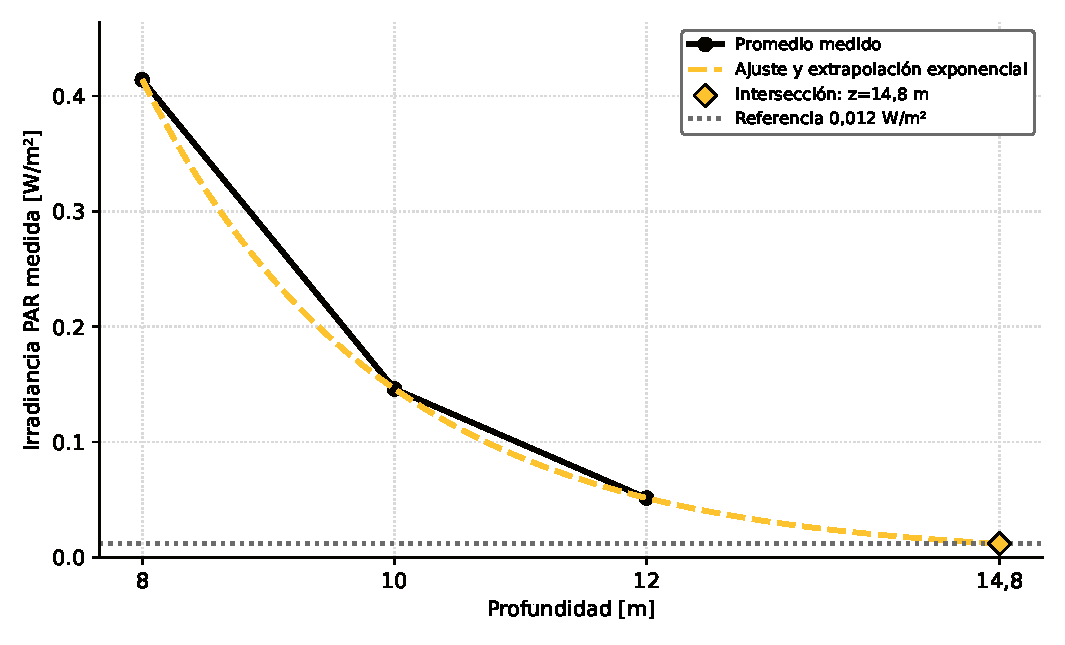
\includegraphics[width=0.88\textwidth]{figures/perfil_profundidad.pdf}
\caption{Perfil del promedio de irradiancia medido a 8, 10 y 12 m y extrapolación del ajuste exponencial hasta \SI{0.012}{\watt\per\square\metre} a 14,8 m (Leclercq \emph{et al.}, 2011; Oppedal \emph{et al.}, 1997).}
\end{figure}

\section{Conclusiones}

El promedio global de las irradiancias medidas fue de \SI{0.2038}{\watt\per\square\metre}, equivalente a 17,0 veces la referencia de \SI{0.012}{\watt\per\square\metre} señalada por Leclercq \emph{et al.} (2011) y Oppedal \emph{et al.} (1997).

La profundidad de 8 m presentó un promedio de \SI{0.4139}{\watt\per\square\metre}, equivalente a 34,5 veces la referencia; a 10 m se obtuvo \SI{0.1461}{\watt\per\square\metre}, equivalente a 12,2 veces; y a 12 m se registró un promedio de \SI{0.0516}{\watt\per\square\metre}, equivalente a 4,3 veces. Los tres valores superan la referencia indicada.

La extrapolación exponencial alcanza el nivel de referencia de \SI{0.012}{\watt\per\square\metre} a 14,8 m de profundidad. Por lo tanto, el perfil promedio mantiene niveles iguales o superiores a la referencia hasta esa profundidad.

Finalmente, de acuerdo con la irradiancia promedio global, los promedios obtenidos a 8, 10 y 12 m y la extrapolación exponencial hasta 14,8 m, se concluye que el sistema de fotoperíodo entrega niveles de irradiancia suficientes respecto de la referencia biológica de \SI{0.012}{\watt\per\square\metre} hasta esa profundidad.

\end{document}
